\chapter{Proses Bisnis dan Pengumpulan Data Fisik}

\section{Proses Bisnis}
Sebelum kita dapat menganalisa untuk perancangan sistem database maka kita membutuhkan beberapa berkas untuk kita analisis dan berkas-berkas tersebut ada dalam proses bisnis pembuatan e-KTP sebagai berikut :
\begin{enumerate}
	\item Pertama, pemohon/warga meminta surat pengantar RT dan RW setempat dengan membawa berkas yaitu Kartu Keluarga asli atau Fotocopy Kartu Keluarga untuk memvalidasi bahwa pemohon/warga terdaftar sebagai Warga Negara Indonesia.
	\begin{figure}[H]
		\centering
		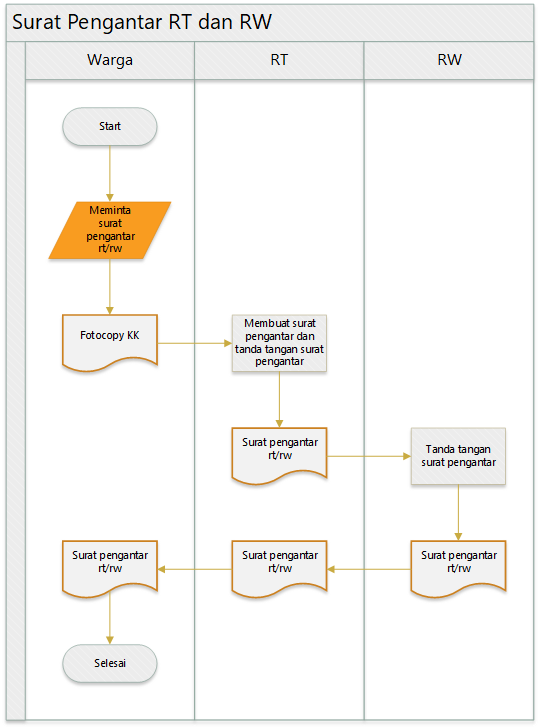
\includegraphics[width=6cm]{figures/suratf.png}
		\caption{Flowmap : Surat Pengantar RT dan RW.}	
	\end{figure}
	\item Kedua, pemohon/warga pergi menuju kelurahan setempat untuk meminta Formulir F-1.21 dengan membara berkas Fotocopy Akta Kelahiran, Fotocopy Kartu Keluarga, dan Surat Pengantar RT dan RW, lalu petugas akan memvalidasi data tersebut sebelum 			         menyerahkan data tersebut kembali beserta dengan Formulir F-1.21.
	\begin{figure}[H]
		\centering
		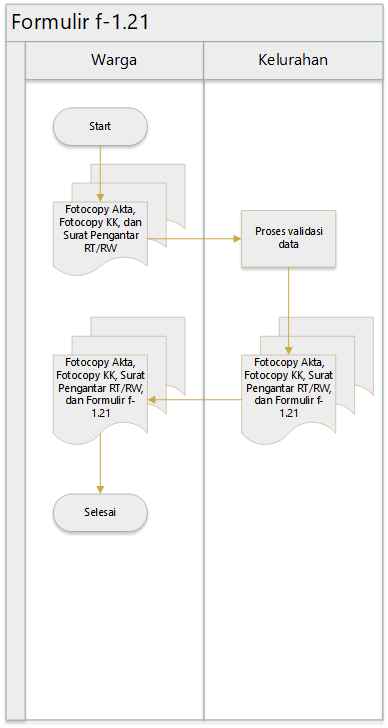
\includegraphics[width=6cm]{figures/formulirf.png}
		\caption{Flowmap : Formulir F-1.21.}	
	\end{figure}
	\item Ketiga, pemohon/warga mengisi Formulir F-1.21 sesuai dengan data diri pemohon/warga.
	\item Keempat, pemohon/warga pergi menuju Kecamatan atau DISDUKCAPIL untuk menyerahkan berkas seperti Fotocopy Akta Kelahiran, Fotocopy Kartu Keluarga, Formulir F-1.21, dan foto 3x4 lalu mengambil nomor antrian.
	\item Kelima, pemohon/warga memasuki ruangan untuk pengambilan beberapa record data seperti Foto, Tanda Tangan, Sidik Jari, dan validasi data pemohon/warga.
	\begin{figure}[H]
		\centering
		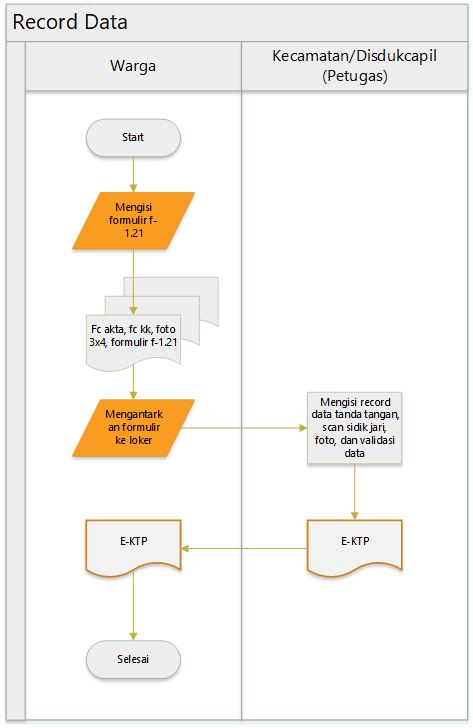
\includegraphics[width=6cm]{figures/recordf.png}
		\caption{Flowmap : Record Data.}	
	\end{figure}
	\item Keenam, pemohon/warga menunggu proses e-KTP jadi sekitar 1 minggu dan dapat diambil dikelurahan atau desa setempat.
\end{enumerate}

\section{Pengumpulan Data Fisik}
Setelah kita mengetahui beberapa langkah proses bisnis dalam pembuatan e-KTP baru, maka kita mendapatkan beberapa berkas fisik yang nantinya akan kita analisis untuk perancangan database, yaitu seperti berikut : 
\begin{enumerate}

	\item Kartu Keluarga
	\begin{figure}[H]
		\centering
		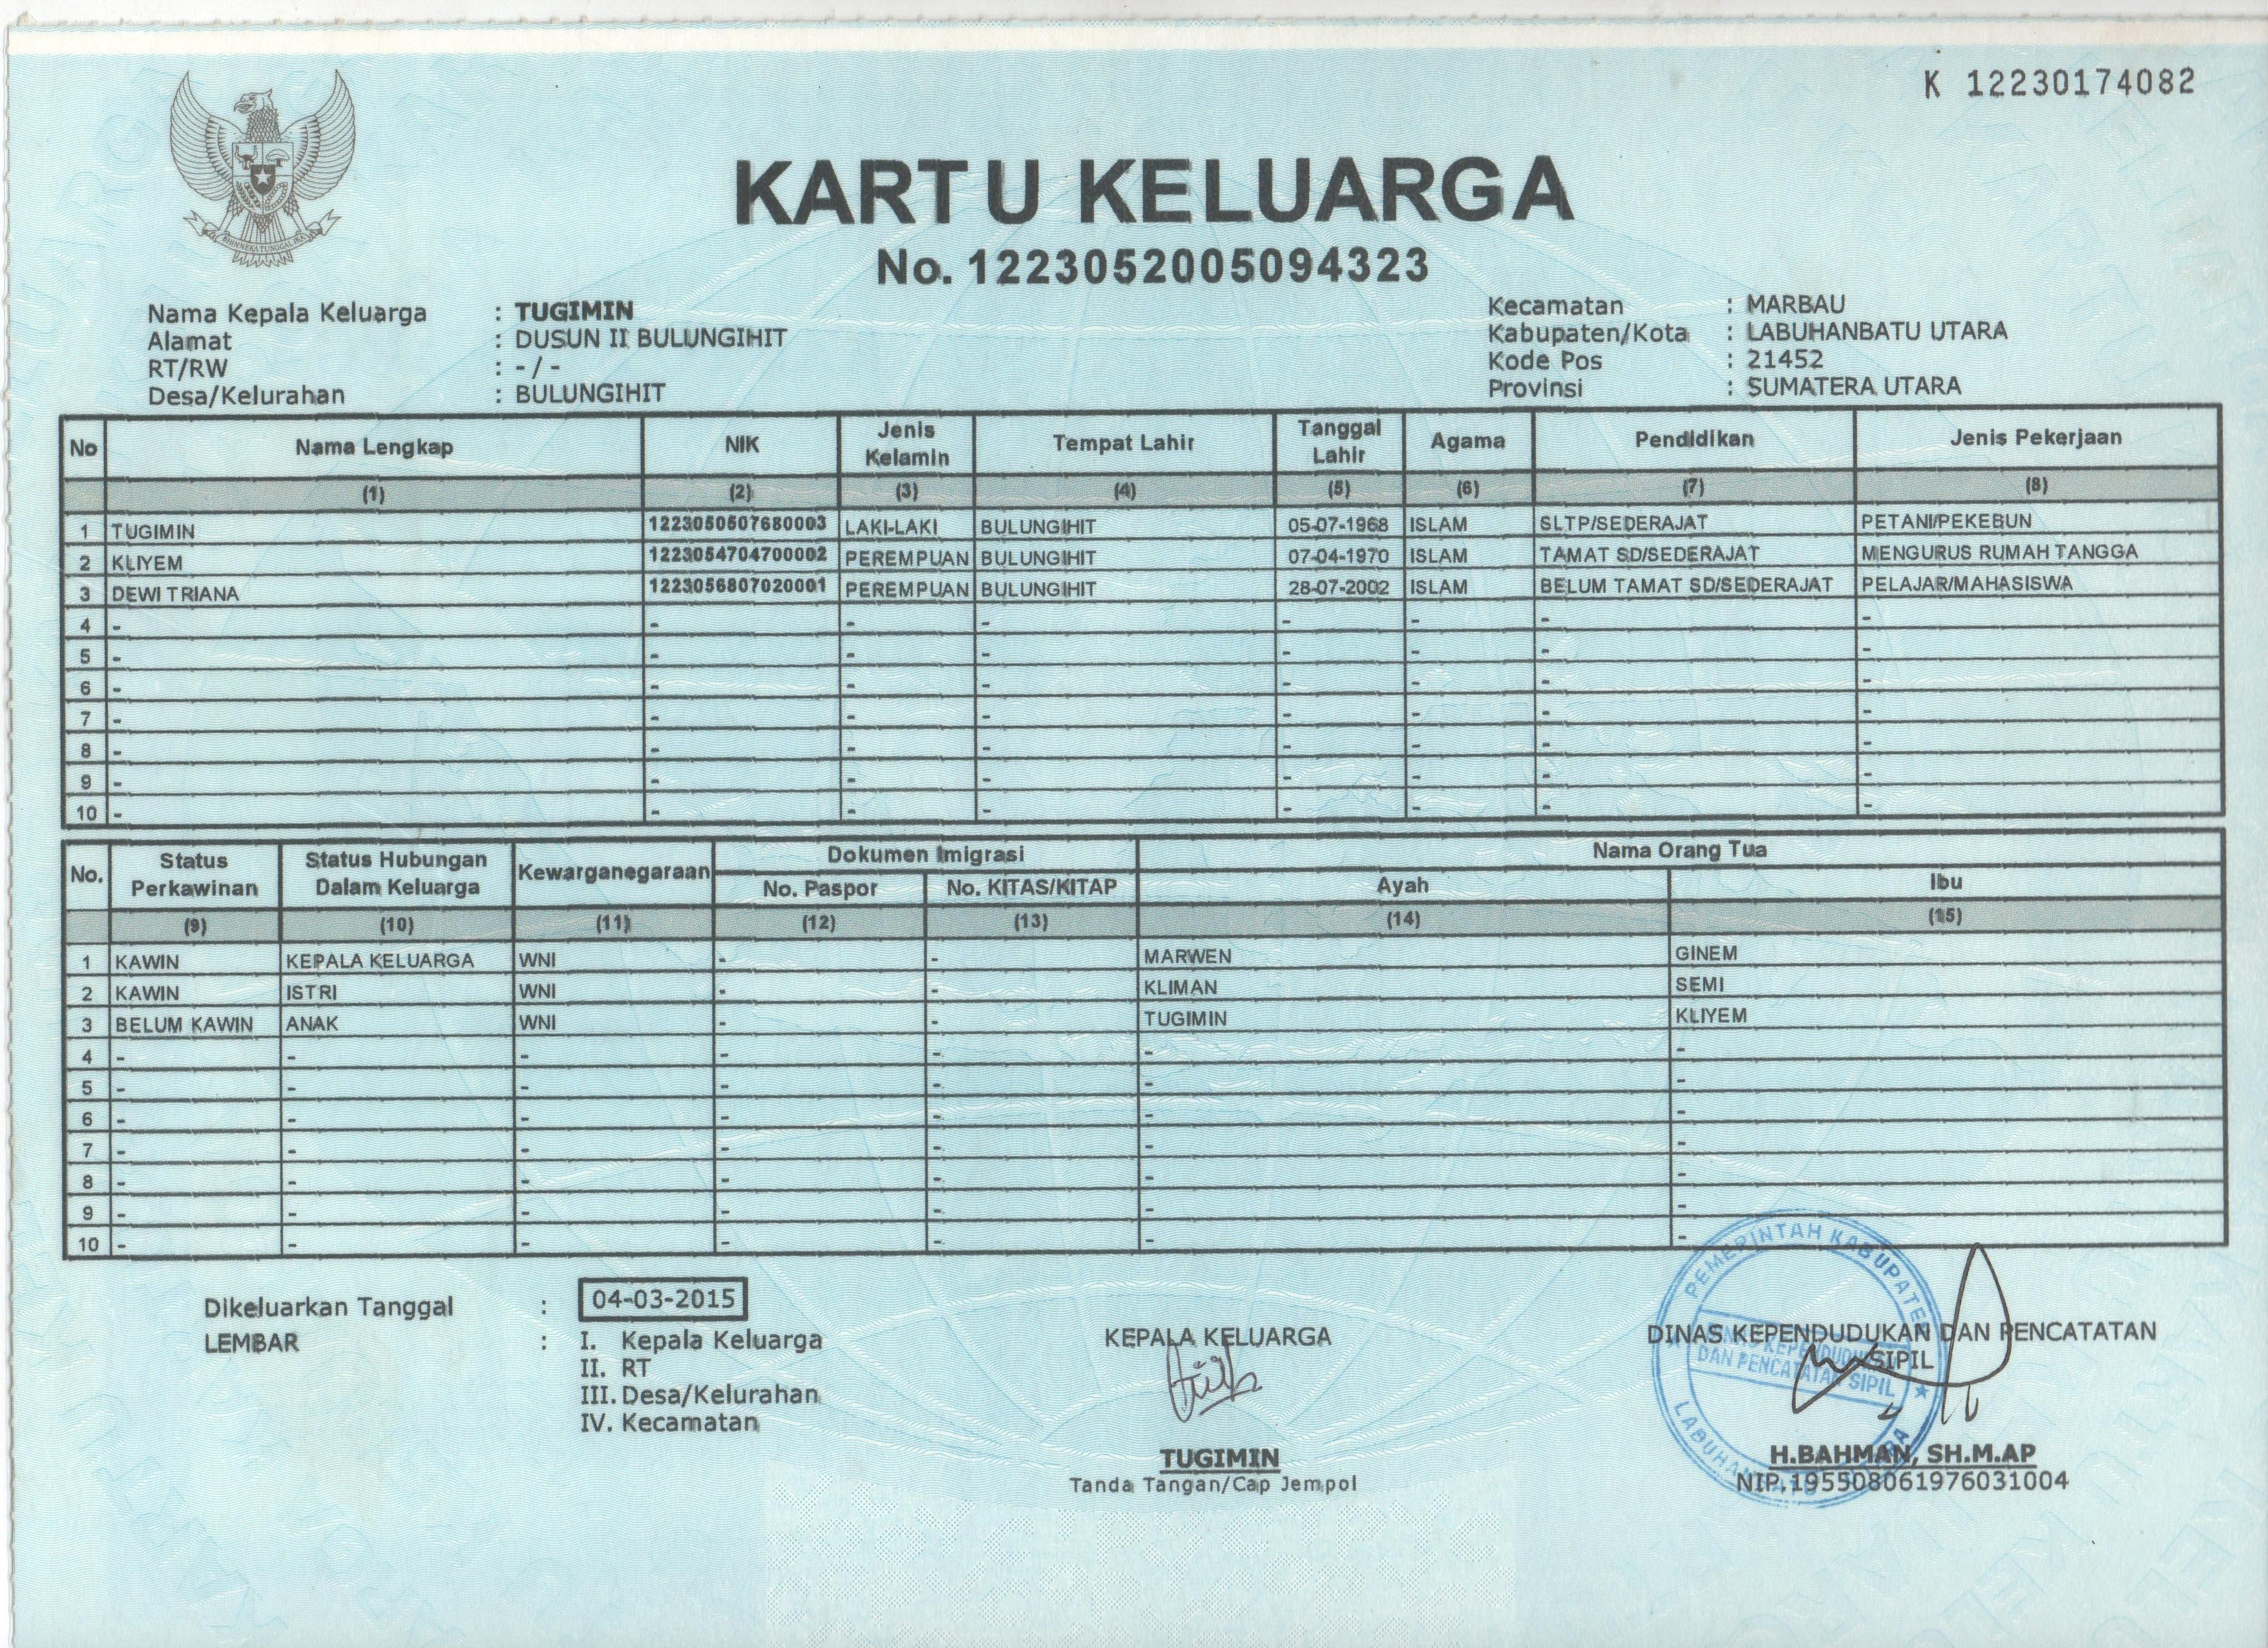
\includegraphics[width=12cm]{figures/kk.jpg}
		\caption{Kartu Keluarga.}	
	\end{figure}

	\item Akta Kelahiran
	\begin{figure}[H]
		\centering
		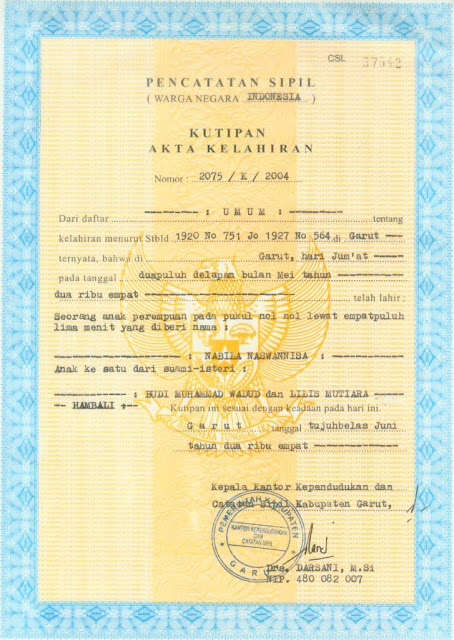
\includegraphics[width=12cm]{figures/akta.jpg}
		\caption{Akta Kelahiran.}	
	\end{figure}

	\item Formulir F-1.21
	\begin{figure}[H]
		\centering
		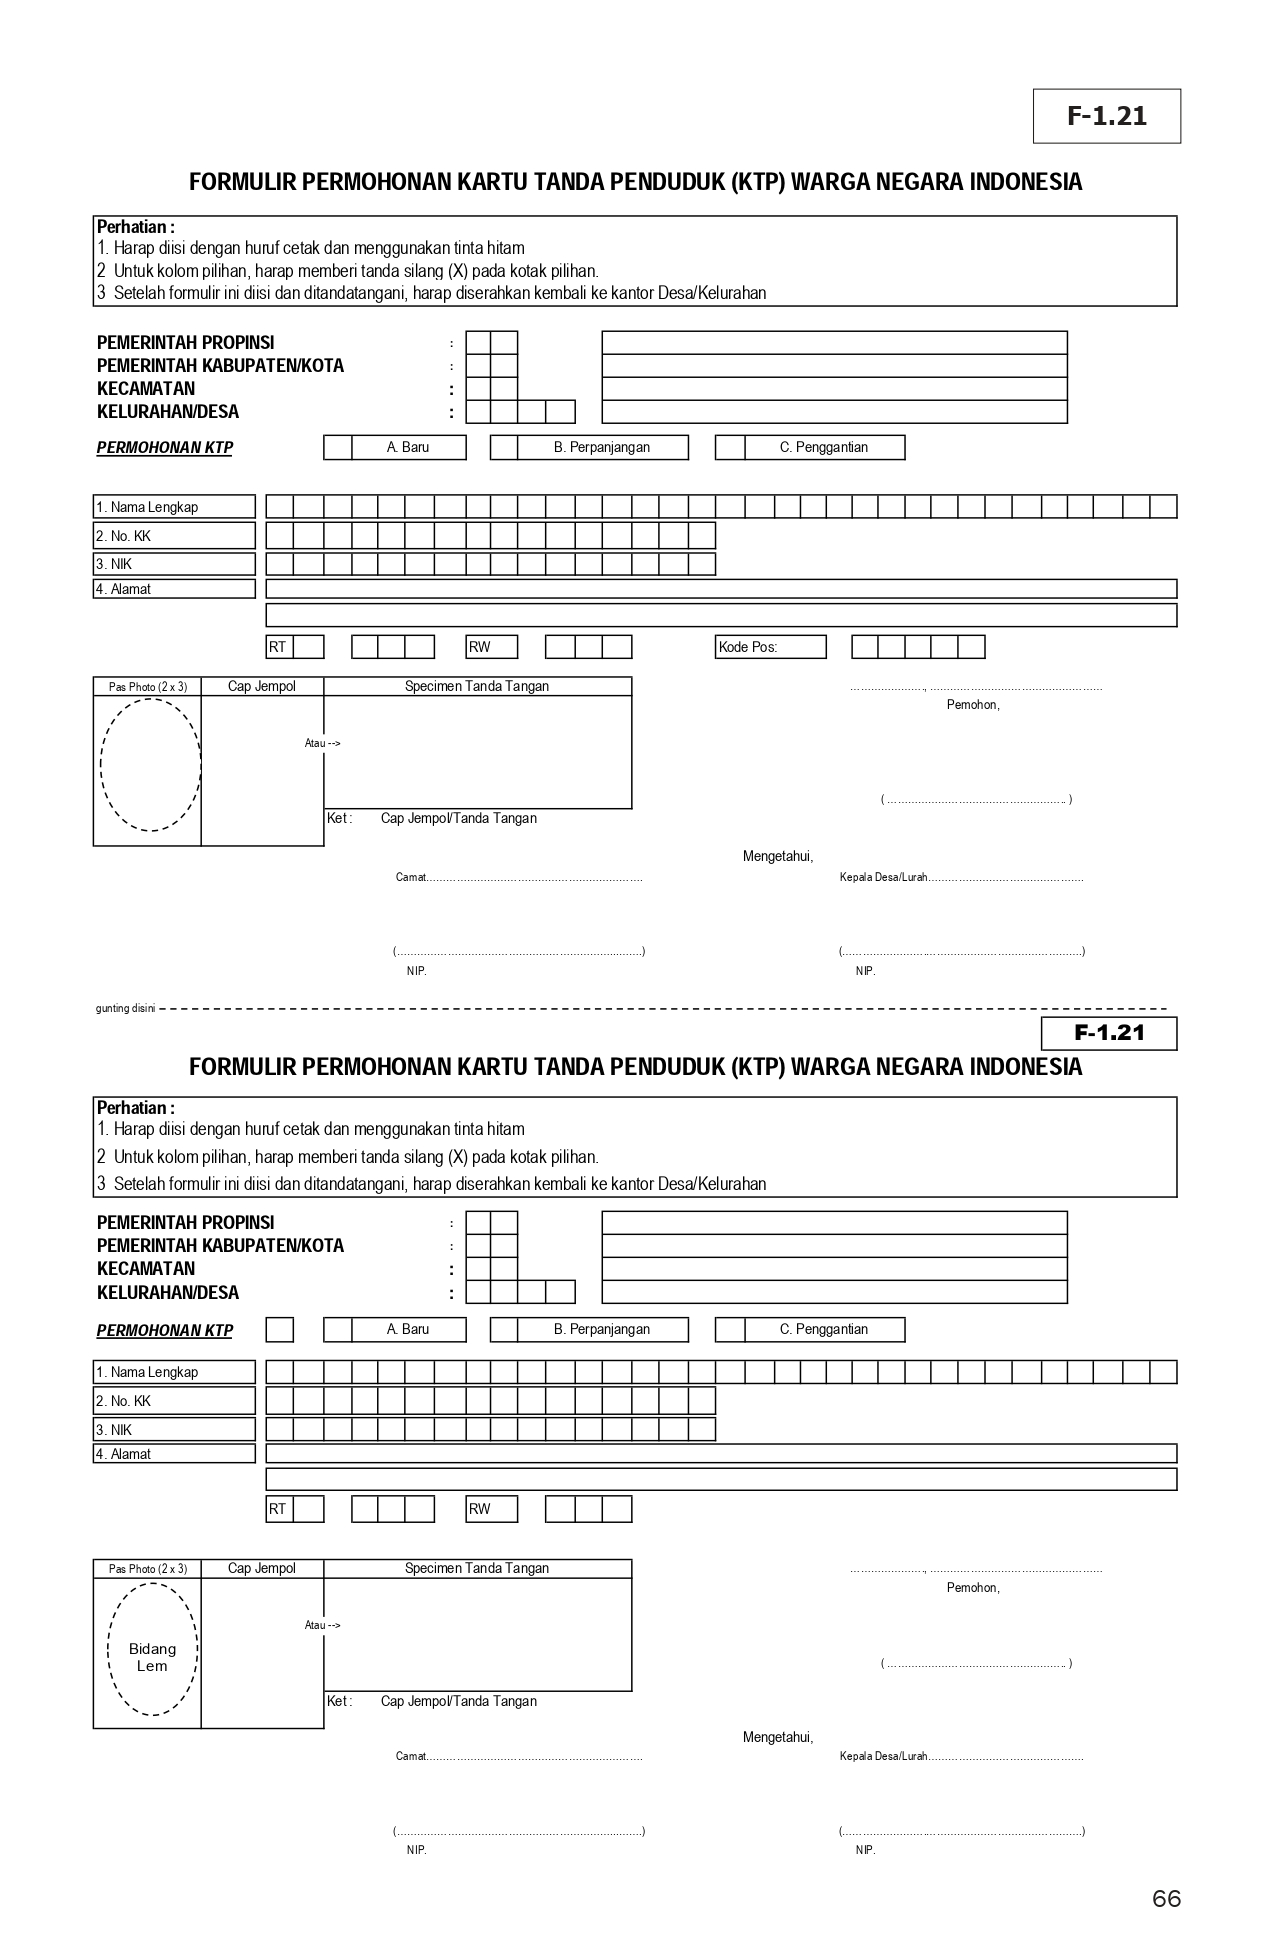
\includegraphics[width=12cm]{figures/formulir.jpg}
		\caption{Formulir F-1.21.}	
	\end{figure}

	\item Surat Pengantar RT dan RW
	\begin{figure}[H]
		\centering
		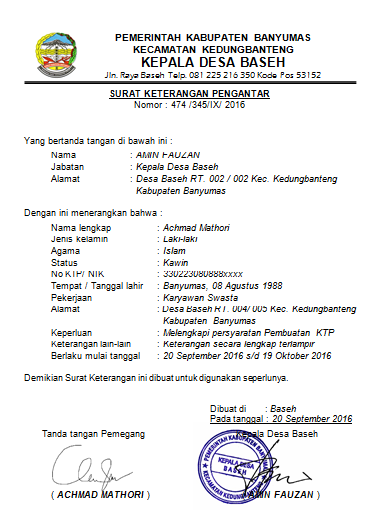
\includegraphics[width=12cm]{figures/surat.png}
		\caption{Surat Pengantar RT dan RW.}	
	\end{figure}

	\item e-KTP
	\begin{figure}[H]
		\centering
		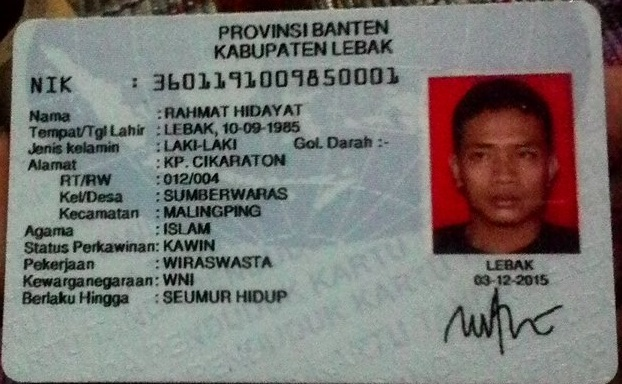
\includegraphics[width=12cm]{figures/ktp.jpg}
		\caption{e-KTP.}	
	\end{figure}

\end{enumerate}